\section{Smart Contract: ExamContract}

Per la realizzazione dello smart contract, è stata utilizzata la piattaforma Ethereum. In particolare, il contratto è stato scritto in Solidity, il linguaggio di programmazione orientato agli oggetti, più diffuso per l'implementazione di contratti intelligenti su varie piattaforme blockchain tra cui Ethereum stessa. In fine, il contratto è stato deployato sulla rete di test Goerli, in quanto Ropsten risulta deprecata dal 21 Gennaio e verrà disabilitata nel Q4 del 2022.\\
\\
Durante l'analisi dei requisiti, ci si è resi conto che nonostante l'utilizzo dell'indirizzo garantisca pseudo-anonimicità, non è particolarmente user-friendly. Per questo, si è deciso di utilizzare un'associazione tra indirizzo pubblico e matricola, permettendo l'utilizzo di quest'ultima per l'inserimento di voti da parte del prof.\\
\\
Nella fase di progettazione, si è deciso di separare il sorgente in due file diversi. Nel primo file, IExamContract.sol, è stata definita l'interfaccia del contratto, definendo metodi, strutture ed eventi. Questa scelta ha permesso di individuare tutte le funzionalità da implementare prima di definirne dettagli. Successivamente, è stato realizzato ExamContract.sol, un'implementazione dell'interfaccia discussa sopra.

\subsection{Controlli sulle dipendenze}
Per rendere più completo il contratto, è stata aggiunta la possibilità di definire propedeuticità a livello di materie e dipendenze tra test della stessa materia.
Dall'analisi dei requisiti, sono stati individuati diversi scenari.

\subsubsection{Materie}
Per quanto riguarda le materie, non sono state rilevate grandi difficoltà.
Una materia può avere delle propedeuticità, ma una volta superate la materia è disponibile per il resto della carriera universitaria.
Prendendo in esempio la propedeuticità:
$$
    Prog1 \rightarrow Prog2
$$
E' possibile definire all'interno di Prog1 una lista di materie che verranno `Sbloccate' al superamento. Per stabilire se una materia è sbloccata o meno, è stato utilizzato un contatore, inizializzato con il numero di materie propedeutiche.
\\
Con questa soluzione, internamente si avrà:
\begin{minted}{python}
prog1 = {counter: 0, unlocks: [prog2]}
prog2 = {counter: 1, unlocks: []}
# Superamento esame di prog1 per lo studente stud1
for unlock in prog1.unlocks:
    stud1.materia(unlock).counter -=1
\end{minted}

\subsubsection{Prove}
Per rendere il contratto più completo, senza però obbligare gli insegnanti ad scegliere fra poche modalità di esame prestabilita,
è stato realizzato un complesso sistema di dipendenze tra le prove. \\
Ogni prova può avere un numero arbitrario di prove che devono essere state superate per permetterne lo svolgimento.
Inoltre è possibile specificare anche quali risultati precedentemente ottenuti verranno invalidati
nel momento in cui la prova viene fallita o anche solo intrapresa. \\
Infine, i risultati di una prova saranno considerati validi solo per il tempo stabilito nella descrizione della stessa
da quanto lo studente lo ha superato, e il voto minimo per considerare la prova superata. \\
\\
La struttura dati utilizzata è così composta:
\begin{minted}{solidity}
    struct Test {
        string name;
        uint256 expiresIn;
        uint8 minMark;
        uint8[][] testIdxRequired;
        uint8[] testIdxReset;
        uint8[] testIdxResetOnTake;
    }
\end{minted}

Sebbene il sistema è sicuramente più complesso di quello che sarebbe lo stretto necessario,
ciò ci permette di realizzare e controllare grafi delle dipendenze anche molto complessi (\autoref{fig:testGraph}).


\begin{figure}
    \centering
    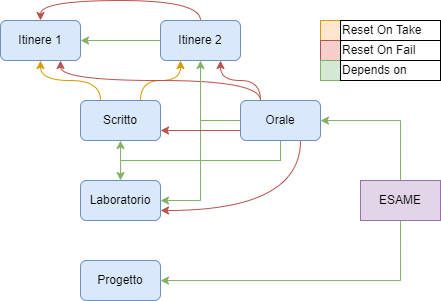
\includegraphics[width=0.75\columnwidth,keepaspectratio]{img/TestGraph.png}
    \caption{Un possibile grafico delle dipendenze tra le prove}
    \label{fig:testGraph}
\end{figure}

\subsection{Tipologie di utenti}
\label{sec:roles}
Sempre durante la fase di progettazione, sono state identificate tre tipologie di utenti:
\begin{itemize}
    \item Admin
    \item Professore
    \item Studente
\end{itemize}

\subsubsection{Admin}
La prima tipologia di utente, corrisponde al creatore del contratto. Quest'ultimo ha la possibilità di definire il nome, le propedeuticità e i relativi CFU delle materie, l'associazione tra matricola ed indirizzo pubblico e la gestione della lista dei professori autorizzati alla verbalizzazione dei test e del voto finale delle singole materie. In generale, è possibile considerare questo account come la componente amministrativa dell'università, per questo motivo ci riferiremo a questo ruolo con il termine `University' nelle figure successive.

\subsubsection{Professore}
Nonostante abbia la capacità di definire le caratteristiche della materie, la definizione dei test spetta alla seconda tipologia di utente, il professore.
Quest'ultimo, dopo aver ricevuto l'autorizzazione da parte dell'admin, può invocare la funzione \texttt{setSubjectTests()}, passando una lista di oggetti \texttt{Test} che verrà discussa successivamente. In \autoref{fig:createSubject} è possibile vedere il diagramma di flusso, con tutti gli attori coinvolti.\\
\\
Il professore ha inoltre la possibilità di proporre un voto finale, tramite la funzione \texttt{setSubjectResults()}, specificando come argomento una lista di coppie \texttt{<Matricola,VotoFinale>}. Il voto finale dovrà essere esplicitamente accettato dallo studente, come descritto in \autoref{fig:registerSubjectVotes}.

\begin{figure}
    \centering
    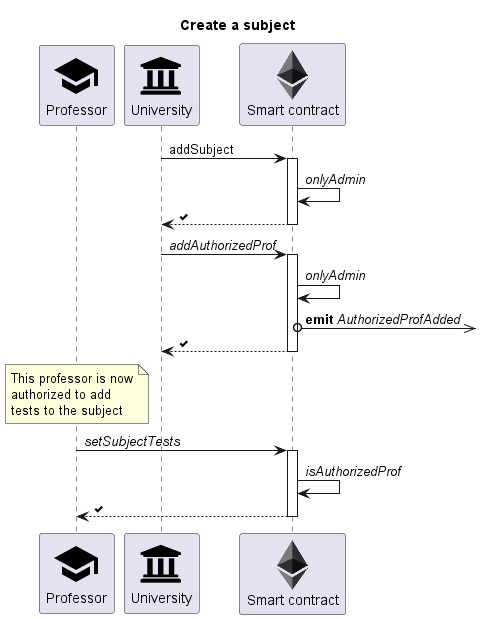
\includegraphics[width=0.70\columnwidth]{img/CreateSubject.png}
    \caption{Diagramma di flusso: `Create a subject'}
    \label{fig:createSubject}
\end{figure}

\begin{figure}
    \centering
    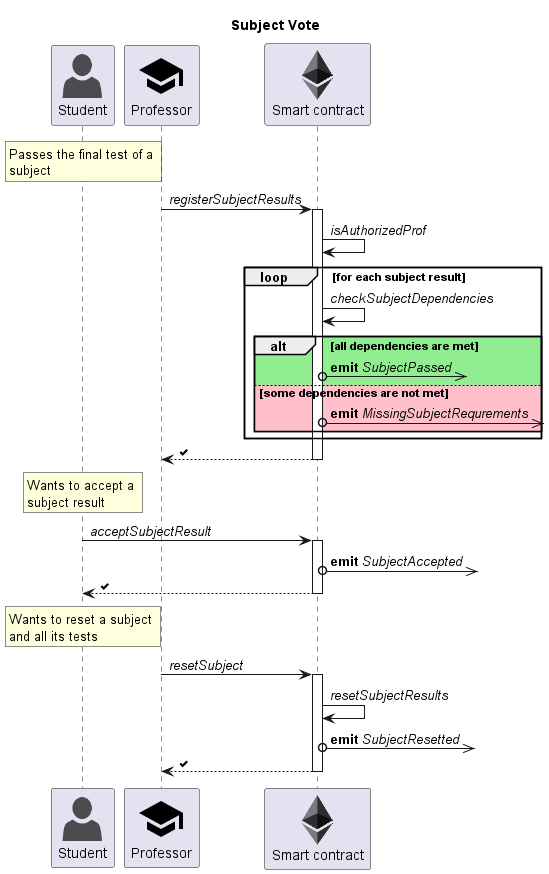
\includegraphics[width=0.85\columnwidth]{img/SubjectVote.png}
    \caption{Diagramma di flusso: `Register subject votes'}
    \label{fig:registerSubjectVotes}
\end{figure}

\pagebreak

\subsubsection{Studente}
L'ultima tipologia di utente progettata è lo studente. E' identificato da una matricola univoca e dal relativo indirizzo pubblico. Affinché un utente venga riconosciuto dal contratto come studente, è necessario che esista l'associazione $\textit{Indirizzo pubblico} \Rightarrow \textit{Matricola}$, aggiunta precedentemente dall'admin.
Sostanzialmente lo studente ha accesso a tre funzioni:
\begin{itemize}
    \item Accettare/Rifiutare la proposta di voto di una materia
    \item Rifiutare il voto di un test
    \item Resettare tutti i test di una materia
\end{itemize}

Si noti che lo studente ho la la possibilità di accettare esplicitamente il voto di una prova.
Aggiungere questa funzionalità si tradurrebbe in transazioni aggiuntive non necessarie. \\
Ricordando infatti che operare su uno \gls{smart-contract} richiede una spesa di gas che si traduce in un utilizzo della currency della blockchain,
è interesse di tutti gli utenti minimizzare il numero di transazioni effettuate. \\
Per questo motivo, è più efficiente assumere che un voto superiore a quello minimo di una prova sia automaticamente accettato,
e permettere allo studente di rifiutare esplicitamente i risultati che non lo soddisfano. \\
\\
Sarebbe anche possibile invertire l'ipotesi e assumere che un test sia rifiutato di default, a prescindere dal voto.
Lo studente dovrebbe quindi manualmente accettare tutti risultati che lo soddisfano. \\
Tuttavia, poiché il fine ultimo è quello di superare la prova, ogni studente si vedrebbe costretto,
nel caso migliore, ad accettare ognuno degli $n$ test. \\
Statisticamente, dunque, il primo metodo riduce al minimo il numero di transazioni necessarie. \\
\\
Lo stesso ragionamento non è invece applicabile per le materie, poiché la scelta di accettare o meno il voto è finale,
ed influenza lo studente per il resto della sua carriera. \\
In virtù di ciò, lo studente è comunque protetto da un insegnante malevolo, poiché quest'ultimo potrebbe solo influenzare
i voti dei test, senza però riuscire ad imporre un voto finale senza il consenso esplicito dello studente.

\begin{figure}
    \centering
    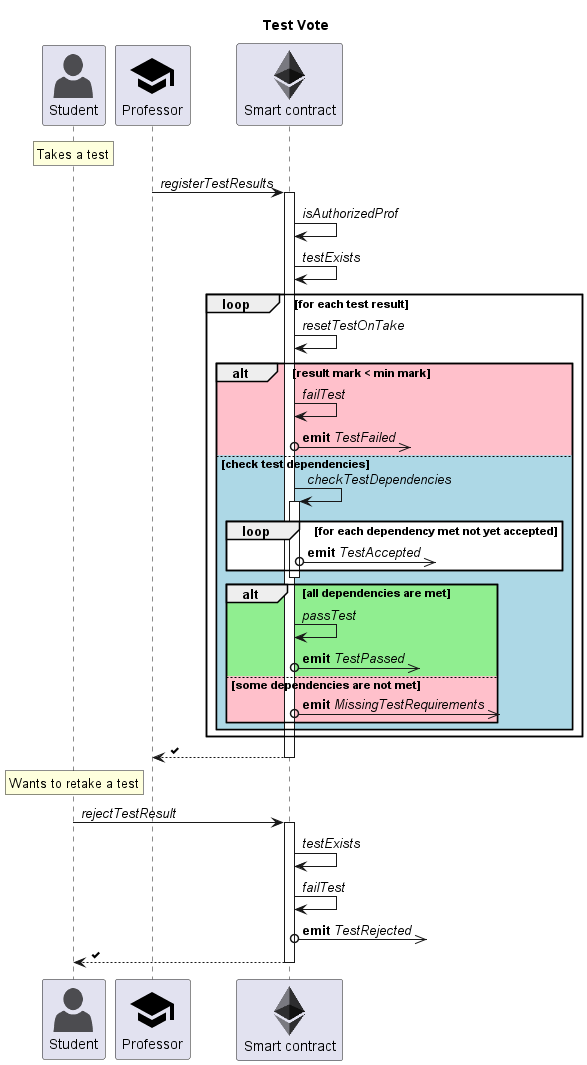
\includegraphics[width=0.75\columnwidth]{img/TestVote.png}
    \caption{Diagramma di flusso: `Register test votes'}
    \label{fig:registerTestVotes}
\end{figure}

\subsection{Implementazione dello smart contract}

Dopo aver individuato e circoscritto i requisiti necessari, è arrivato il momento dell'implementazione dello \gls{smart-contract}.

\subsubsection{Strumenti di sviluppo}

Lo sviluppo dello smart contract si è svolto in locale, utilizzando il framework hardhat \cite{soft:hardhat}.
Si tratta di un ambiente di sviluppo per \gls{smart-contract} di \gls{ethereum} dotato di moltissimi componenti
che consentono di svolgere operazioni come il debugging, la compilazione e il testing di \gls{smart-contract}. \\
\\
Una feature aggiuntiva realizzata dal plugin @typechain/hardhat \cite{soft:typechain_hardhat} è la creazione automatica di
classi proxy e funzioni che descrivono accuratamente i metodi dello \gls{smart-contract},
che è poi possibile importare ed utilizzare in qualsiasi file typescript, semplificando l'interazione con lo \gls{smart-contract}. \\
\\
hardhat si occupa anche del deployment dello \gls{smart-contract} su Ethereum. \\
Fornendo una chiave privata associata ad un account con sufficiente credito e un nodo \gls{rpc-api} a cui collegarsi,
è estremamente facile realizzare un semplice script (\autoref{cod:deployment}) che si occupi di distribuire lo \gls{smart-contract} sulla blockchain scelta.

\inputminted{typescript}{../contracts/scripts/deployExam.ts}
\captionof{listing}{Script che si occupa del deployment dello \gls{smart-contract} su \gls{ethereum} \label{cod:deployment}}

\subsubsection{Test}

Il framework utilizzato mette a disposizione anche una serie di metodologie per poter testare facilmente e velocemente lo \gls{smart-contract}. \\
Utilizzando un'apposita estensione della libreria chai \cite{soft:chai}, combinata con una blockchain simulata in locale da hardhat
è possibile effettuare il deploy dello \gls{smart-contract} e verificare che tutti i suoi metodi si comportino come previsto. \\
I test variano dal controllo del valore di ritorno del metodo invocato, al verificare che lo stato del contratto sia stato alterato nella maniera corretta,
e anche assicurarsi che venga prodotta l'eccezione prevista su input invalidi. \\
Mettendo insieme tutti i test, è stata raggiunta una \href{https://app.codecov.io/gh/TendTo/Exam-Manager}{copertura del 100\%} del codice \footnote{https://app.codecov.io/gh/TendTo/Exam-Manager}. \\
\\
Si ricordi però che una copertura del 100\% non assicura l'assenza di errori imprevisti, ma indica unicamente che, durante i test,
tutte le righe di codice sono state toccate almeno una volta dell'esecuzione.
La protezione da eventuali bug e regressioni è assicurata solo rispetto ai casi che sono stati effettivamente testati. \\
\\
Segue qualche esempio di test utilizzato:
\begin{minted}{typescript}
    it("Should add a student", async function () {
      const studId = 1;
      await contract.addStudent(stud1, studId);
      expect(await contract.studentIds(stud1)).to.equal(studId);
    });

    it("Should revert with 'UnauthorizedProfessorError'", async function () {
      await expect(contract.registerTestResults(prog1.id, 0, []))
      .to.be.revertedWithCustomError(
        contract,
        Errors.UnauthorizedProfessorError
      );
    });
\end{minted}

\subsection{Strutture dati}

Per la gestione dei dati all'interno della blockchain lo \gls{smart-contract} utilizza un approccio ibrido. \\
Viene salvato in maniera persistente, e quindi occupa spazio di archiviazione nel contratto, solo ciò di cui lo stesso ha bisogno per
svolgere i controlli di validazione previsti. \\
Al contrario, tutto il resto viene reso pubblico ed immutabile attraverso lo strumento degli \gls{event-log},
emessi nel momento in cui avviene l'evento corrispondente. \\
Questo approccio è più economico rispetto allo storage tradizionale, ma impedisce al contratto stesso di recuperare i dati emessi in precedenza. \\
\\
Lo storage tradizionale è utilizzato per le strutture dati:
\begin{minted}{solidity}
    //Admins's address
    address public immutable admin;
    //SubjectID -> Subject
    mapping(uint256 => Subject) public subjects;
    //StudentAddress -> StudentId
    mapping(address => uint256) public studentIds;
    //StudentID -> (SubjectID, subjectCareer)
    mapping(uint256 => StudentCareer) public careers;
\end{minted}

Sono invece previsti i seguenti eventi per produrre gli \gls{event-log} corrispondente:

\begin{minted}[fontsize=\footnotesize]{solidity}
    event TestPassed(uint256 indexed subjectId, uint8 indexed testIdx, uint256 indexed studentId, uint8 mark);
    event TestFailed(uint256 indexed subjectId, uint8 indexed testIdx, uint256 indexed studentId, uint8 mark);
    event TestAccepted(uint256 indexed subjectId, uint8 indexed testIdx, uint256 indexed studentId, uint8 mark);
    event TestRejected(uint256 indexed subjectId, uint8 indexed testIdx, uint256 indexed studentId);
    event MissingTestRequirements(uint256 indexed subjectId, uint8 indexed testIdx, uint256 indexed studentId);
    event TestResetted(uint256 indexed subjectId, uint8 indexed testIdx, uint256 indexed studentId);
    event SubjectPassed(uint256 indexed subjectId, uint256 indexed studentId, uint8 mark);
    event SubjectAccepted(uint256 indexed subjectId, uint256 indexed studentId, uint8 mark);
    event SubjectResetted(uint256 indexed subjectId, uint256 indexed studentId);
    event MissingSubjectRequrements(uint256 indexed subjectId, uint256 indexed studentId);
    event AuthorizedProfAdded(uint256 subjectId, address indexed profAddr);
    event AuthorizedProfRemoved(uint256 subjectId, address indexed profAddr);
\end{minted}
